\documentclass{beamer}
\usetheme{Copenhagen}

\usepackage{lmodern}
\usepackage{tikz}
\usetikzlibrary{arrows}
\usetikzlibrary{decorations.markings}

\title{Marsupials}
\subtitle{Scientific computing - 372}
\author{Sheldon Deacon 20039867}
\institute{Stellenbosch University}

\begin{document}


%-------------------------------------------------------------------------------
\begin{frame}
	\titlepage
\end{frame}
%-------------------------------------------------------------------------------
\begin{frame}
	\frametitle{Overview}
	\tableofcontents[currentsection]
\end{frame}
%-------------------------------------------------------------------------------
\section{Marsupials}
\begin{frame}
%Did not have enough info on simple.wikipeadia so got some more from 
%(normal)https://en.wikipedia.org/wiki/Marsupial	

\frametitle{Marsupials}
	Marsupials are any members of the mammalian infraclass Marsupialia.
	\newline \newline
	All extant marsupials are endemic to Australasia and the Americas. 
	A distinctive characteristic common to these species is that most of
	the young are carried in a pouch.
\end{frame}

\begin{frame}
	Well-known marsupials include kangaroos, wallabies, koalas, possums, 
	opossums, wombats, and Tasmanian devils. Some lesser-known marsupials
	are the potoroo and the quokka.
	
	\begin{block}{Paragraph 4}
		Marsupials represent the clade originating from the last common 
		ancestor of extant metatherians. Like other mammals in the 
		Metatheria, they give birth to relatively undeveloped young that 
		often reside in a pouch located on their mothers abdomen for a
		certain amount of time.
	\end{block}

	The word marsupial comes from marsupium, the technical term for the
	abdominal pouch. It, in turn, is borrowed from Latin and ultimately from
	the ancient Greek, which means "pouch."
\end{frame}
%-------------------------------------------------------------------------------
\section{Reproduction}
\begin{frame}
	\frametitle{Reproduction}
	Marsupials give birth to living babies. The babies are called \textit{joeys}. 
	The babies feed on milk. Their babies are born very small.
 	\begin{equation*}
		T_n(x) = \frac{n!}{2\pi i} \oint \frac{e^{x(e^t-1)}}{t^{n+1}}dt.
	\end{equation*}
 	\\
	\begin{equation*}
		Pr[|S_n - E_n| > t] < 2 \ exp \left( -\frac{t^2/2}{V_n+C\cdot t/3} \right)
	\end{equation*}
\end{frame}

\begin{frame}
List of marsupials:
	\begin{itemize}
		\item Bandicoots	
		\item Kangaroos
		\item Koalas
		\item Tasmanian Devil
	\end{itemize}
\end{frame}
%-------------------------------------------------------------------------------
\section{Biogeography}
\begin{frame}
	\frametitle{Biogeography}
	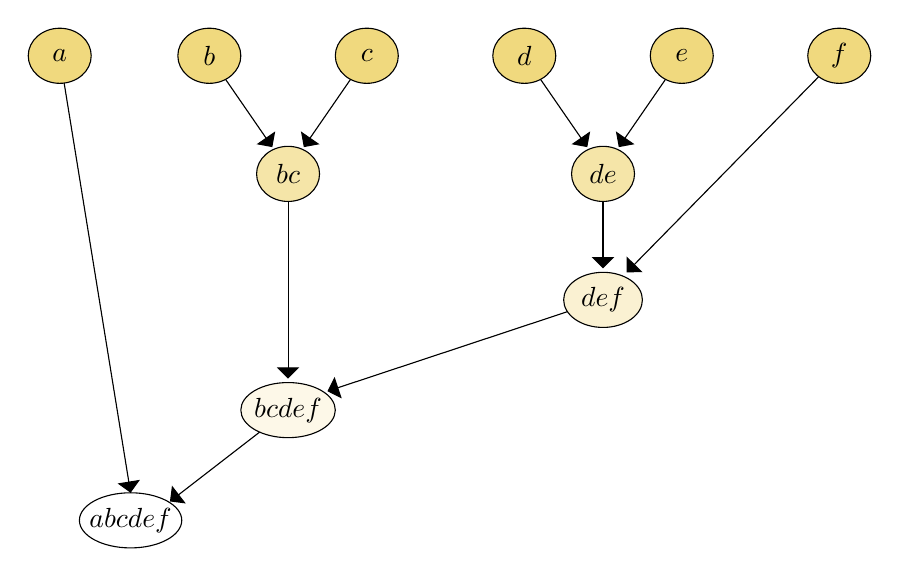
\begin{tikzpicture}
		\definecolor{mycolor1}{RGB}{240,217,126}
		\definecolor{mycolor2}{RGB}{245,229,168}
		\definecolor{mycolor3}{RGB}{250,241,210}
		\definecolor{mycolor4}{RGB}{253,248,232}

		\draw[draw=black,-triangle 90,fill=black] (0.1,6) -- (1,0.45);
		\draw[draw=black,-triangle 90,fill=black] (2,6) -- (2.8,4.84);
		\draw[draw=black,-triangle 90,fill=black] (4,6) -- (3.2,4.84);
		\draw[draw=black,-triangle 90,fill=black] (6,6) -- (6.8,4.84);
		\draw[draw=black,-triangle 90,fill=black] (8,6) -- (7.2,4.84);
		\draw[draw=black,-triangle 90,fill=black] (10,6) -- (7.3,3.25);

		\draw[draw=black,-triangle 90,fill=black] (3,4.5) -- (3,1.9);
		\draw[draw=black,-triangle 90,fill=black] (7,4.5) -- (7,3.3);

		\draw[draw=black,-triangle 90,fill=black] (7,2.9) -- (3.5,1.74);

		\draw[draw=black,-triangle 90,fill=black] (3,1.5) -- (1.5,0.34);


		\draw[fill=mycolor1] (0.1,6) ellipse (0.4cm and 0.35cm) node {$a$};
		\draw[fill=mycolor1] (2,6) ellipse (0.4cm and 0.35cm) node {$b$};
		\draw[fill=mycolor1] (4,6) ellipse (0.4cm and 0.35cm) node {$c$};
		\draw[fill=mycolor1] (6,6) ellipse (0.4cm and 0.35cm) node {$d$};
		\draw[fill=mycolor1] (8,6) ellipse (0.4cm and 0.35cm) node {$e$};
		\draw[fill=mycolor1] (10,6) ellipse (0.4cm and 0.35cm) node {$f$};

		\draw[fill=mycolor2] (3,4.5) ellipse (0.4cm and 0.35cm) node {$bc$};
		\draw[fill=mycolor2] (7,4.5) ellipse (0.4cm and 0.35cm) node {$de$};
		
		\draw[fill=mycolor3] (7,2.9) ellipse (0.5cm and 0.35cm) node {$def$};
	
	
		\draw[fill=mycolor4] (3,1.5) ellipse (0.6cm and 0.35cm) node {$bcdef$};

	
		\draw (1,0.1) ellipse (0.65cm and 0.35cm) node {$abcdef$};


\end{tikzpicture}
\end{frame}

%-------------------------------------------------------------------------------
\section{List of Marsupials}

\begin{frame}
	\frametitle{List of Marsupials}
	The extinct genus \textit{Yalkaparidon} (Order Yalkaparidontia) is a bizarre fossil 
	found in the Oligocene/Miocene deposits of Riversleigh, NE Australia. 
	Its teeth are so strange that palaeontologists call it a 'Thingodont'.
	\newline \newline
	The borhyaenids and the sabertooth \textit{Thylacosmilus} are no longer considered
	to be marsupials. They are sparassodont metatherians, the sister group of
	the marsupials.
\end{frame}

%-------------------------------------------------------------------------------
\section{Related pages}
\begin{frame}
	\frametitle{Related pages}
    	Great American Interchange and Monotreme
\end{frame}
%-------------------------------------------------------------------------------
\end{document}
